\chapter{Misc}
\newpage
\subsubsection*{Covenant Schema}
\begin{table}[h]
  \centering
  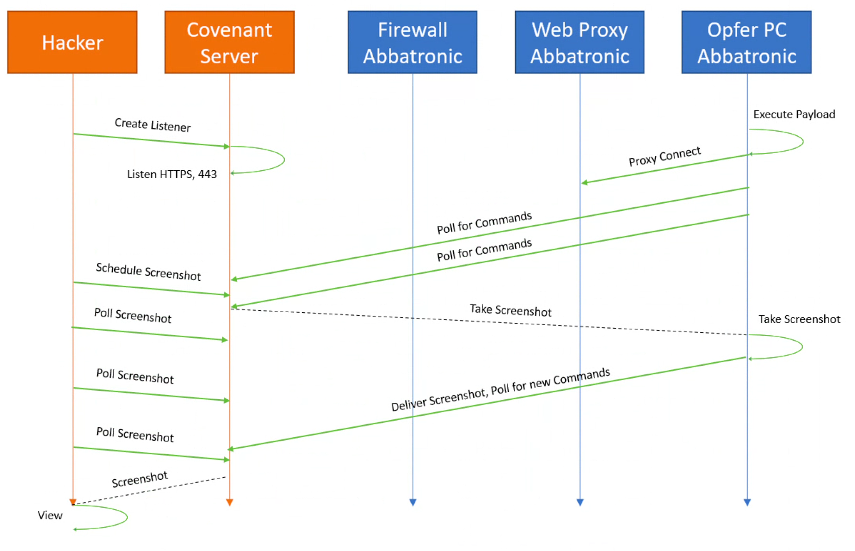
\includegraphics[width=\textwidth]{resources/zzz_covenant_example.png}
  \caption{Covenant Schema}
\end{table}

\subsection{Windows Persistence}

\begin{enumerate}
    \item Windows System Persistence
    \begin{itemize}
        \item Registry modifications
        \begin{itemize}
            \item Run and RunOnce keys
            \item Services registry entries
            \item Explorer shell extensions
            \item Winlogon helper DLLs
        \end{itemize}
        \item Task scheduling mechanisms
        \begin{itemize}
            \item Windows Task Scheduler
            \item At jobs (legacy)
            \item WMI event subscriptions
        \end{itemize}
        \item Startup locations abuse
        \begin{itemize}
            \item Startup folders (user/system)
            \item Application auto-start locations
            \item Shell startup items
        \end{itemize}
    \end{itemize}
    \item Active Directory Persistence
    \begin{itemize}
        \item Group Policy Objects (GPOs)
        \begin{itemize}
            \item Startup/shutdown scripts
            \item Scheduled tasks deployment
            \item Software installation policies
        \end{itemize}
        \item Domain-level techniques
        \begin{itemize}
            \item Service Principal Names (SPNs)
            \item Security Support Provider registration
            \item Group Policy template modifications
        \end{itemize}
        \item Account-based methods
        \begin{itemize}
            \item Shadow credentials
            \item Domain backup operators
            \item Delegation rights modifications
        \end{itemize}
    \end{itemize}
\end{enumerate}


\subsection*{Yara Polymorphic Virus}
It's not meant to detect polymorphic viruses
\begin{enumerate}
    \item Decrypt Routine Detection
    \begin{itemize}
        \item Common decryption operations identification
        \item Characteristic instruction sequences
        \item CPU register usage patterns analysis
        \item Typical sequence: XOR operations, counter increments, loop structures
    \end{itemize}

    \item Cryptographic Constants Identification
    \begin{itemize}
        \item Static initialization vectors
        \item Common S-box values detection
        \item Key schedule constants analysis
    \end{itemize}

    \item Behavioral Pattern Recognition
    \begin{itemize}
        \item Entry point characteristics analysis
        \item Memory allocation patterns
        \item API call sequences monitoring
        \item Process injection indicators
    \end{itemize}

    \item Structure Analysis
    \begin{itemize}
        \item Section size anomalies
        \item Entry point variations
        \item File structure inconsistencies
        \item Header modification patterns
    \end{itemize}

    \item Pattern Matching Techniques
    \begin{itemize}
        \item Wildcard pattern implementation
        \item Flexible byte matching
        \item Variable offset handling
        \item Instruction sequence variations
    \end{itemize}

    \item Statistical Methods
    \begin{itemize}
        \item Entropy calculation
        \item Size anomaly detection
        \item Header validation
        \item Byte frequency analysis
    \end{itemize}
\end{enumerate}

\subsection*{Cyber Security Jobs}
\begin{itemize}
    \item \textbf{Penetration Tester}: A security professional who legally and systematically probes an organization's systems, networks, and applications for vulnerabilities. They simulate targeted attacks using various tools and techniques, document their findings, and provide detailed reports on security weaknesses along with recommendations for remediation. Their goal is to identify and help fix security flaws before malicious actors can exploit them.

    \item \textbf{Red Teamer}: Similar to penetration testers but operating with a broader scope and more sophisticated approach. Red teamers simulate full-scale attacks using multiple vectors including technical exploitation, social engineering, and physical security testing. They typically work in teams and emulate real threat actors' tactics, techniques, and procedures (TTPs) to test an organization's complete security posture, including its detection and response capabilities. Their objective is to help organizations understand how they would fare against actual advanced persistent threats.

    \item \textbf{Digital Forensics Investigator (Police)}: A law enforcement specialist who analyzes digital evidence to solve crimes. They recover and examine data from computers, mobile devices, and other digital storage media using specialized forensic tools while maintaining proper chain of custody. Their work includes analyzing malware, recovering deleted files, examining network logs, and documenting their findings for use in legal proceedings. Their goal is to gather and present digital evidence that can stand up in court.

    \item \textbf{Incident Responder}: A cybersecurity professional who leads the charge when security incidents occur. They analyze security alerts, determine the scope and impact of breaches, contain threats, eradicate malicious presence from systems, and help restore normal operations. They also document incidents, conduct post-incident analysis, and develop recommendations to prevent similar incidents in the future. Their primary objective is to minimize damage and reduce recovery time during security incidents.

    \item \textbf{Threat Actor}: Also known as malicious actors or attackers, these are individuals or groups who actively attempt to exploit vulnerabilities in systems and networks for various motives including financial gain, espionage, activism, or disruption. They can range from opportunistic criminals to state-sponsored groups using sophisticated techniques. While not a legitimate occupation, understanding threat actors is crucial for cybersecurity professionals to better defend against their methods and anticipate their actions.
\end{itemize}